\documentclass[12pt]{article}
\usepackage[margin=0.5in,top=0.5in,bottom=0.5in]{geometry}
\usepackage{amsmath}
\usepackage{indentfirst}
\usepackage{scrextend}
\usepackage{graphicx}
\usepackage{wrapfig}
\usepackage{multicol}
\graphicspath{{images/}}

\title{\textbf{\underline{Assignment 4 Report}}}
\author{Anoop (2015CS10265)}

\begin{document}
\pagenumbering{gobble}
\maketitle

\section*{\underline{K-Means with Scikit-Learn}}
\subsection*{Parts (i) and (ii)}
\begin{addmargin}[0.3in]{0in}
\begin{tabbing}
n\_init \qquad \= = 10 \qquad \qquad \= Train Accuracy \= 0.34279 \\
n\_clusters \> = 20 \> Test Accuracy \> = 0.34437 \\
max\_iter \> = 300 \\
\end{tabbing}
\end{addmargin}
\subsection*{Part (iii)}
\begin{addmargin}[0.3in]{0in}
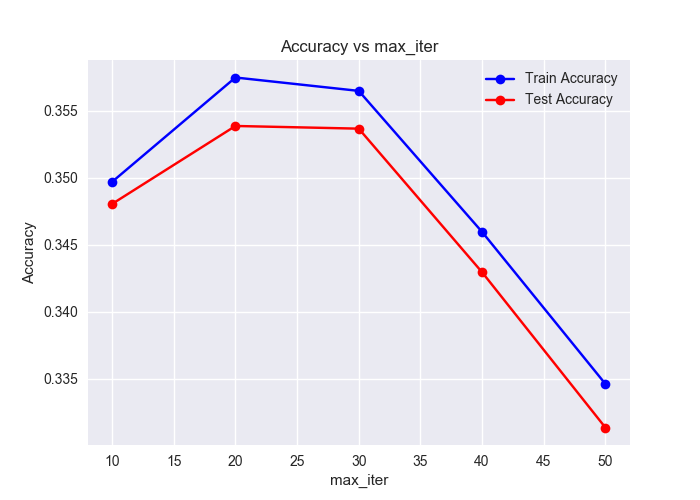
\includegraphics[width=0.8\textwidth]{kmeans.png} \\
The accuracy peaks when max\_iter is set to 20. This is one of the local minima that the K-Means converges to. We can infer this from the fact that later on when max\_iter is set to 300 (in the previous part), the accuracy increases as compared to other settings.
\end{addmargin}

\section*{\underline{SVM with Dimensionality Reduction using PCA}}
\begin{addmargin}[0.3in]{0in}
\begin{multicols}{2}
\underline{Parameters}:
\begin{tabbing}
    kernel \quad \= = `rbf' \\
    gamma \> = [1e-2, 1e-3] \\
    C \> = [0.01, 0.1, 1, 10, 100] \\
\end{tabbing}
Best Setting - C = 10 and gamma = 1e-2 \\
\begin{tabbing}
    Train Accuracy \= = 0.69376 \\
    Test Accuracy \> = 0.64714 \\
\end{tabbing}
\underline{Parameters}:
\begin{tabbing}
    kernel \quad \= = `linear' \\
    C \> = [0.01, 0.1, 1, 10, 100] \\ \\
\end{tabbing}
Best Setting - C = 1 \\
\begin{tabbing}
    Train Accuracy \= = 0.68145 \\
    Test Accuracy \> = 0.63538 \\
\end{tabbing}
\end{multicols}
\end{addmargin}
\begin{addmargin}[0.3in]{0in}
\underline{Hyperparameter Tuning} - 3-Fold Grid Search Cross-Validation \\ \\
SVM takes too long to train even after dimensionality reduction. Normalization is necessary for fast convergence. SVM gives decent performance on both train and test data.
\end{addmargin}

\section*{\underline{Neural Networks with Keras}}
\begin{addmargin}[0.3in]{0in}
\underline{Parameters}:
\begin{tabbing}
Number of Hidden Units \= = [2, 5, 10, 20, 50, 100, 200, 300, 500, 1000] \\
Number of Epochs \> = 50 \\
Batch Size \> = 64 \\
\end{tabbing}
\underline{Hyperparameter Tuning} - 3-Fold Grid Search Cross-Validation \\ \\
Best Setting - Number of Hidden Units = 5 \\
Best Model is trained for 100 more epochs after Cross-Validation \\
\begin{tabbing}
Train Accuracy \= = 0.81200 \\
Test Accuracy \> = 0.66855 \\
\end{tabbing}
\end{addmargin}

\section*{\underline{Convolutional Neural Networks with Keras}}
\begin{addmargin}[0.3in]{0in}
\underline{Parameters}:
\begin{tabbing}
Number of Filters (3 X 3) \= = 32 \\
Number of Hidden Units \> = 50 (Fully Connected Layer) \\
Number of Epochs \> = 100 \\
Batch Size \> = 32 \\
\end{tabbing}
\begin{tabbing}
Train Accuracy \= = 0.95317 \\
Test Accuracy \> = 0.81761 \\
\end{tabbing}
\end{addmargin}

\section*{\underline{Comparison of Models}}
\begin{addmargin}[0.3in]{0in}
\begin{itemize}
    \item \underline{K-Means}
        \begin{itemize}
            \item Training Time - 3s per model (Approx. 20s for CV)
            \item Poor training and test accuracies.
        \end{itemize}
    \item \underline{SVM with PCA}
        \begin{itemize}
            \item Training Time - 15 mins per model (Approx. 4 hrs for CV)
            \item Decent training and test accuracies.
        \end{itemize}
    \item \underline{Neural Networks}
        \begin{itemize}
            \item Training Time - 2s per epoch (Approx. 1 hr for CV) + 5 mins for extra 100 epochs [Used GPU]
            \item Very good training accuracy but comparitively poor test accuracy. Significant Overfitting.
        \end{itemize}
    \item \underline{Convolutional Neural Networks}
        \begin{itemize}
            \item Training Time - 5s per epoch (Approx. 10 mins for 100 epochs) [Used GPU]
            \item Very good training accuracy but comparitively poor test accuracy. Significant Overfitting. \\
        \end{itemize}
\end{itemize}
CNN performs well on the test data though it overfits. It takes comparitively lesser time to train than an SVM. Hyperparameter tuning in CNNs is difficult as compared to other models.
\end{addmargin}

\section*{\underline{Best Model (Submitted in the Competition)}}
\begin{addmargin}[0.3in]{0in}
\textbf{\underline{Key ideas used}: }
\begin{itemize}
    \item Ensemble of CNNs is used to predict the test labels. Prediction of the ensemble is simply the most frequent prediction.
    \item Individual CNN is trained for 25 epochs. After 5 epochs, a snapshot of the model along with the test predictions are stored. This gives 5 different models per architecture. \\
    \underline{Note}: Only those architectures are considered which give very good train accuracy ($\approx$ 0.90) after first 5 epochs.
    \item Data Augmentation using in-built Image Preprocessing techniques in Keras in one of the architectures (Not utilized completely).
\end{itemize}
\textbf{\underline{Note}: Individual architectures are not described here. Check the code for complete details of the architectures. Individual Test Accuracies are not calculated.} \\
\begin{tabbing}
Train Accuracy \= = 0.93114 \\
Test Accuracy \> = 0.92502 \\
\end{tabbing}
\end{addmargin}

\end{document}